% ----------------------------------------------------------
% Capítulo 5 -- Implementação
% ----------------------------------------------------------
\chapter{Implementação}\label{cap:implementacao}

Este capítulo apresenta a materialização da solução em \textit{software}. Descreve o ambiente utilizado no desenvolvimento, a organização da equipe, a estrutura da aplicação, a implementação de seus componentes, a integração dos módulos em ambiente de execução e os testes realizados. Em seguida, confronta os resultados obtidos com os requisitos do sistema, estima o custo de operação da plataforma e registra as limitações conhecidas da versão desenvolvida.

\section{Ambiente de Desenvolvimento}

O código-fonte foi versionado em um repositório Git hospedado no GitHub. O \autoref{quadro-ambiente} relaciona as ferramentas e tecnologias que compõem o ambiente de desenvolvimento.

{\ABNTEXfontereduzida
\renewcommand{\arraystretch}{1.25}
\begin{xltabular}{\textwidth}{|>{\raggedright\arraybackslash}p{4.4cm}|>{\raggedright\arraybackslash}X|}
\multicolumn{2}{@{}c@{}}{\quadrolongocaption{Ambiente de desenvolvimento.}\label{quadro-ambiente}} \\[0.3em]
\hline
\textbf{Elemento} & \textbf{Especificação} \\
\hline
\endfirsthead
\multicolumn{2}{@{}r@{}}{\textit{(continuação)}} \\
\hline
\textbf{Elemento} & \textbf{Especificação} \\
\hline
\endhead
\multicolumn{2}{@{}r@{}}{\textit{(continua)}} \\
\endfoot
\endlastfoot
Ambiente de desenvolvimento integrado & IntelliJ IDEA (servidor) e editor de código para a aplicação \textit{web} \\
\hline
Servidor & Java Development Kit 21; Gradle 9.4.1, por meio do \textit{wrapper} do projeto \\
\hline
Aplicação \textit{web} & Node.js 20; gerenciador de pacotes npm; servidor de desenvolvimento Vite 5 \\
\hline
Banco de dados & MySQL local (desenvolvimento) e H2 em memória (testes automatizados) \\
\hline
Testes de API & Postman e documentação interativa Swagger UI \\
\hline
Navegadores & Google Chrome e Mozilla Firefox \\
\hline
Versionamento e integração contínua & Git e GitHub, com fluxos automatizados no GitHub Actions \\
\hline
Qualidade de código & SonarCloud e JaCoCo \\
\hline
\end{xltabular}
\legend{Fonte: Autoria própria (2026).}
}

A API foi configurada com três perfis de execução, selecionados por variável de ambiente, que isolam as configurações de cada ambiente, conforme o \autoref{quadro-perfis}.

{\ABNTEXfontereduzida
\renewcommand{\arraystretch}{1.25}
\begin{xltabular}{\textwidth}{|>{\raggedright\arraybackslash}p{2.5cm}|>{\raggedright\arraybackslash}p{4.9cm}|>{\raggedright\arraybackslash}X|}
\multicolumn{3}{@{}c@{}}{\quadrolongocaption{Perfis de execução da API.}\label{quadro-perfis}} \\[0.3em]
\hline
\textbf{Perfil} & \textbf{Banco de dados} & \textbf{Uso} \\
\hline
\endfirsthead
\multicolumn{3}{@{}r@{}}{\textit{(continuação)}} \\
\hline
\textbf{Perfil} & \textbf{Banco de dados} & \textbf{Uso} \\
\hline
\endhead
\multicolumn{3}{@{}r@{}}{\textit{(continua)}} \\
\endfoot
\endlastfoot
test & H2 em memória, criado pelo Hibernate e carregado por \textit{script} de inicialização & Execução dos testes automatizados e experimentação local, sem dependência de servidor de banco. \\
\hline
dev & MySQL local & Desenvolvimento e testes manuais com dados persistentes. \\
\hline
prod & MySQL no Amazon RDS & Ambiente de produção na nuvem. \\
\hline
\end{xltabular}
\legend{Fonte: Autoria própria (2026).}
}

As informações sensíveis e dependentes do ambiente — credenciais do cliente OAuth, duração do \textit{token}, origens autorizadas para CORS, servidor e remetente de e-mail — são lidas de variáveis de ambiente. Na aplicação \textit{web}, o endereço da API, o identificador do cliente Google e o fuso horário da instituição são definidos por arquivos de ambiente distintos para desenvolvimento e produção.

Nos perfis que utilizam MySQL, o esquema do banco não é gerado automaticamente. Cada alteração do modelo de dados é acompanhada de um \textit{script} SQL próprio, versionado no repositório e identificado pelo requisito correspondente, aplicado de forma controlada aos bancos de desenvolvimento e de produção.

O projeto foi desenvolvido por uma equipe de seis integrantes, com atribuições distribuídas de acordo com as competências de cada um. O \autoref{quadro-equipe} resume a função e as principais contribuições de cada integrante, com base nas atribuições definidas pela equipe e no histórico de contribuições do repositório.

{\ABNTEXfontereduzida
\renewcommand{\arraystretch}{1.25}
\begin{xltabular}{\textwidth}{|>{\raggedright\arraybackslash}p{4.5cm}|>{\raggedright\arraybackslash}p{3.9cm}|>{\raggedright\arraybackslash}X|}
\multicolumn{3}{@{}c@{}}{\quadrolongocaption{Atribuições dos integrantes da equipe.}\label{quadro-equipe}} \\[0.3em]
\hline
\textbf{Integrante} & \textbf{Função} & \textbf{Principais atribuições} \\
\hline
\endfirsthead
\multicolumn{3}{@{}r@{}}{\textit{(continuação)}} \\
\hline
\textbf{Integrante} & \textbf{Função} & \textbf{Principais atribuições} \\
\hline
\endhead
\multicolumn{3}{@{}r@{}}{\textit{(continua)}} \\
\endfoot
\endlastfoot
Camilly Freire & Desenvolvimento \textit{front-end} e experiência do usuário & Experiência do usuário e estruturação de rotas por perfil e \textit{layouts} base da aplicação \textit{web}. \\
\hline
Joseane Lelis de Sousa & Desenvolvimento \textit{back-end}, análise de testes e documentação & Correções no servidor apontadas pela análise estática, análise dos testes e documentação do projeto. \\
\hline
Matheus Soares & Desenvolvimento \textit{front-end} e experiência do usuário & Implementação das telas da aplicação \textit{web}: gestão de instituições e alunos, trilhas e sínteses, curadoria de \textit{links}, painel, panorama, perfil e leque de possibilidades. \\
\hline
Olívia Helena de Lima & Banco de dados, \textit{front-end} e plano de testes & Integração contínua e análise de qualidade (GitHub Actions, JaCoCo e SonarCloud), telas do profissional de orientação, agendamentos com o Google Agenda e plano de testes. \\
\hline
Pedro Yoshiaki Freitas Nohara & Desenvolvimento \textit{back-end}, documentação e implantação & API do leque de possibilidades, do histórico de jornadas e dos \textit{feedbacks}, correções de concorrência e de tratamento de erros, implantação na AWS e documentação do projeto. \\
\hline
Victor Rodrigues de Barros & Desenvolvimento \textit{back-end} e banco de dados & Base da API — autenticação e segurança, gestão de instituições, turmas e usuários, painel, sínteses, agendamentos, relatórios e e-mails —, testes automatizados e banco de dados. \\
\hline
\end{xltabular}
\legend{Fonte: Autoria própria (2026).}
}

O código-fonte do servidor e da aplicação \textit{web}, os \textit{scripts} SQL, as definições dos fluxos de integração contínua e a documentação do projeto estão reunidos no repositório público \url{https://github.com/VictorB4rros/synccarreira}. O trabalho seguiu um fluxo baseado em ramificações: cada requisito ou correção foi desenvolvido em um ramo próprio, integrado ao ramo principal por meio de \textit{pull request} revisado pelos demais integrantes. A cada \textit{pull request}, o GitHub Actions compila o servidor e a aplicação \textit{web}, executa os testes automatizados e envia o relatório de cobertura e o código para análise estática no SonarCloud.

\section{Estrutura da Aplicação}

O repositório reúne, em diretórios separados, a documentação do projeto, o código do servidor e o código da aplicação \textit{web}, além das definições dos fluxos de integração contínua. A \autoref{fig_pacotes} apresenta o diagrama de pacotes da aplicação, com as dependências entre os pacotes de cada parte.

\begin{figure}[!htbp]
    \centering
    \caption{Diagrama de pacotes do SyncCarreira.}
    \label{fig_pacotes}
    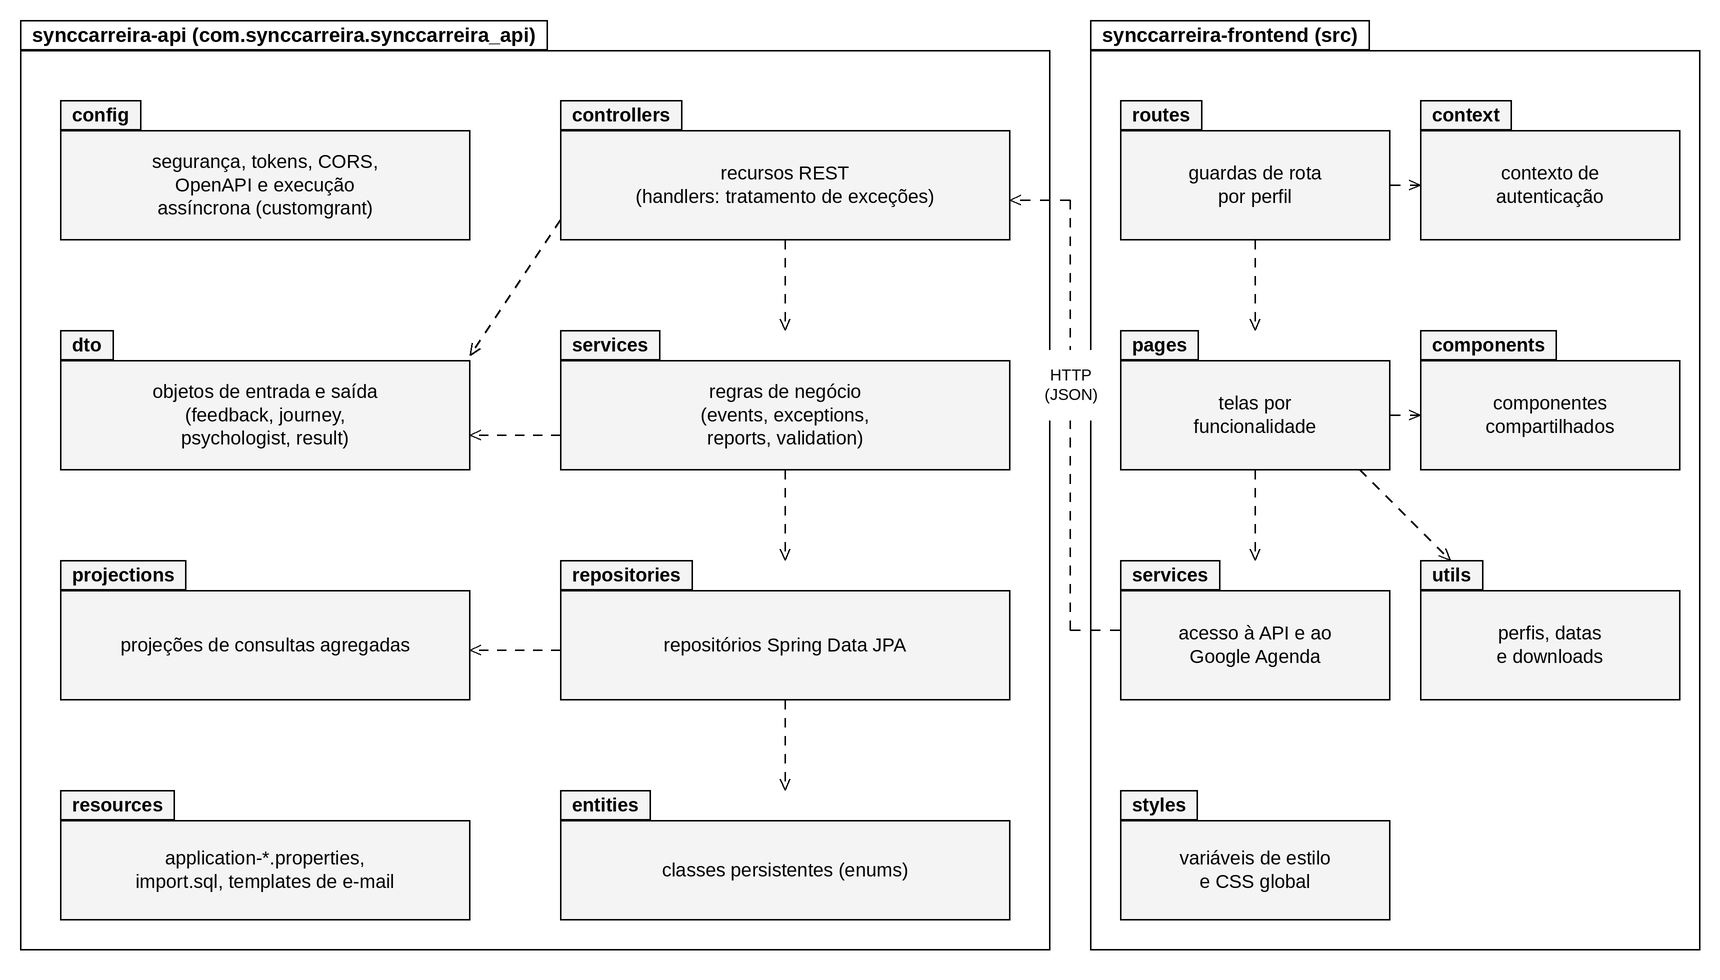
\includegraphics[width=\textwidth]{img/fig-cap5-pacotes.png}
    \legend{Fonte: Autoria própria (2026).}
\end{figure}

No servidor, os pacotes seguem as camadas da arquitetura. O pacote controllers depende dos serviços e dos objetos de transferência; o pacote services concentra as regras de negócio e se subdivide em eventos, exceções, geradores de relatórios e validadores; o pacote repositories acessa as entidades e utiliza projeções para as consultas agregadas do painel; e o pacote config reúne as configurações de segurança, de emissão de \textit{tokens}, de CORS, de documentação e de execução assíncrona. As entidades são utilizadas por todas as camadas. Os recursos do servidor incluem os arquivos de configuração por perfil, o \textit{script} de carga inicial e os modelos HTML das mensagens eletrônicas. Os testes automatizados replicam a estrutura de pacotes do código de produção e contam com fábricas de objetos para a montagem dos cenários.

Na aplicação \textit{web}, as páginas são agrupadas por funcionalidade — autenticação, trilhas, jornada, resultado, perfil, painel do profissional de orientação, gestão e agendamentos — e utilizam os serviços de acesso à API e ao Google Agenda, os componentes compartilhados e as funções utilitárias. O pacote routes define as rotas e as guardas de acesso por perfil, apoiado no contexto de autenticação.

\section{Implementação dos Componentes}

Esta seção destaca os aspectos técnicos mais relevantes da implementação de cada componente.

\subsection{Autenticação e autorização}

A emissão de \textit{tokens} foi implementada com o Spring Authorization Server. Como a concessão por senha do proprietário do recurso não é oferecida nativamente pelo \textit{framework}, foi desenvolvida uma concessão personalizada, composta por um conversor, que extrai o e-mail e a senha da requisição, um provedor de autenticação, que valida as credenciais contra a senha armazenada com BCrypt, e um \textit{token} de autenticação próprio. O \textit{token} JWT gerado recebe as declarações de perfis de acesso e de nome de usuário, e o servidor de recursos converte essas declarações em autoridades do Spring Security, utilizadas nas regras de autorização de cada rota.

\subsection{Validação e tratamento de erros}

Os dados de entrada são validados por anotações declarativas nos objetos de transferência e por validadores personalizados, como o de unicidade de e-mail e o de dígitos verificadores do CNPJ. Um manipulador global converte as exceções em respostas padronizadas, contendo o código de situação HTTP, a mensagem e, nos erros de validação, a lista de campos rejeitados.

\subsection{Jornada, trilhas e sínteses}

A liberação das trilhas é calculada a cada acesso a partir da ordem sequencial, das respostas e das sínteses registradas, sem armazenar uma situação que pudesse se tornar inconsistente. O registro de respostas substitui a resposta anterior à mesma questão e é repetido automaticamente quando ocorre bloqueio no banco de dados por requisições simultâneas. Na interface, as questões em escala Likert são apresentadas com quatro opções, sem ponto neutro, o que incentiva o posicionamento do aluno. Ao registrar a última síntese, o serviço de histórico grava a jornada concluída, com uma cópia em formato JSON das questões, respostas, sínteses e \textit{links}, que permite consultá-la e exportá-la posteriormente mesmo após o início de um novo ciclo.

\subsection{Leque de possibilidades}

O cálculo do leque foi isolado em um componente específico, que compara as quatro áreas do conhecimento pelo percentual da pontuação obtida em relação à máxima possível de cada área, destaca as de maior percentual, inclusive em caso de empate, e seleciona as subáreas e carreiras correspondentes. As subáreas e carreiras foram carregadas no banco de dados com base na classificação de áreas de formação adotada pelo Inep, a Cine Brasil \cite{inep2019cine}. O mesmo componente é utilizado na conclusão da jornada, na tela de resultado, no registro em PDF e na seleção dos \textit{links} exibidos na trilha de Informação.

\subsection{Painel, relatórios e documentos}

O painel do profissional de orientação é montado com consultas agregadas por instituição, que retornam, em poucas consultas, a quantidade de questões respondidas e as sínteses de todos os alunos, evitando uma consulta por aluno. Os relatórios de turma e individuais são gerados em planilha com a biblioteca Apache POI, e o registro de cada jornada concluída é gerado em PDF com a biblioteca OpenPDF.

\subsection{Notificações por e-mail}

As mensagens são compostas a partir de modelos HTML processados pelo Thymeleaf e enviadas com uma versão alternativa em texto puro, o que melhora a entrega pelos filtros de mensagens indesejadas. O envio é disparado por eventos tratados somente após a confirmação da transação, executado de forma assíncrona e repetido automaticamente em caso de falha temporária, exceto quando a falha é de autenticação no servidor de e-mail. O endereço e o nome do remetente são configuráveis, o que permitiu utilizar um serviço de envio transacional com o domínio próprio do projeto.

\subsection{Aplicação web}

A aplicação \textit{web} utiliza uma instância única do cliente HTTP com interceptadores que anexam o \textit{token} às requisições e tratam, de forma centralizada, as respostas de sessão expirada e de acesso negado. As guardas de rota consultam o contexto de autenticação para restringir cada tela ao perfil correspondente. A integração com o Google Agenda utiliza o modelo de \textit{token} do Google Identity Services: o profissional de orientação autoriza o acesso à própria agenda, e a aplicação cria eventos com geração de \textit{link} de videoconferência e envio de convites aos alunos, mantendo o \textit{token} do Google apenas em memória e cancelando o evento caso a API não aceite o registro da sessão.

\section{Integração dos Módulos}

Em execução, os módulos comunicam-se exclusivamente por meio de interfaces de rede. A aplicação \textit{web} é carregada pelo navegador e consome a API por requisições HTTPS com o \textit{token} JWT no cabeçalho de autorização; a API aceita requisições de navegador apenas das origens configuradas. A API acessa o banco de dados por JDBC e envia mensagens por SMTP, enquanto a integração com o Google Agenda é feita diretamente pelo navegador. A \autoref{fig_implantacao} apresenta o diagrama de implantação do ambiente de produção.

\begin{figure}[!htbp]
    \centering
    \caption{Diagrama de implantação do SyncCarreira.}
    \label{fig_implantacao}
    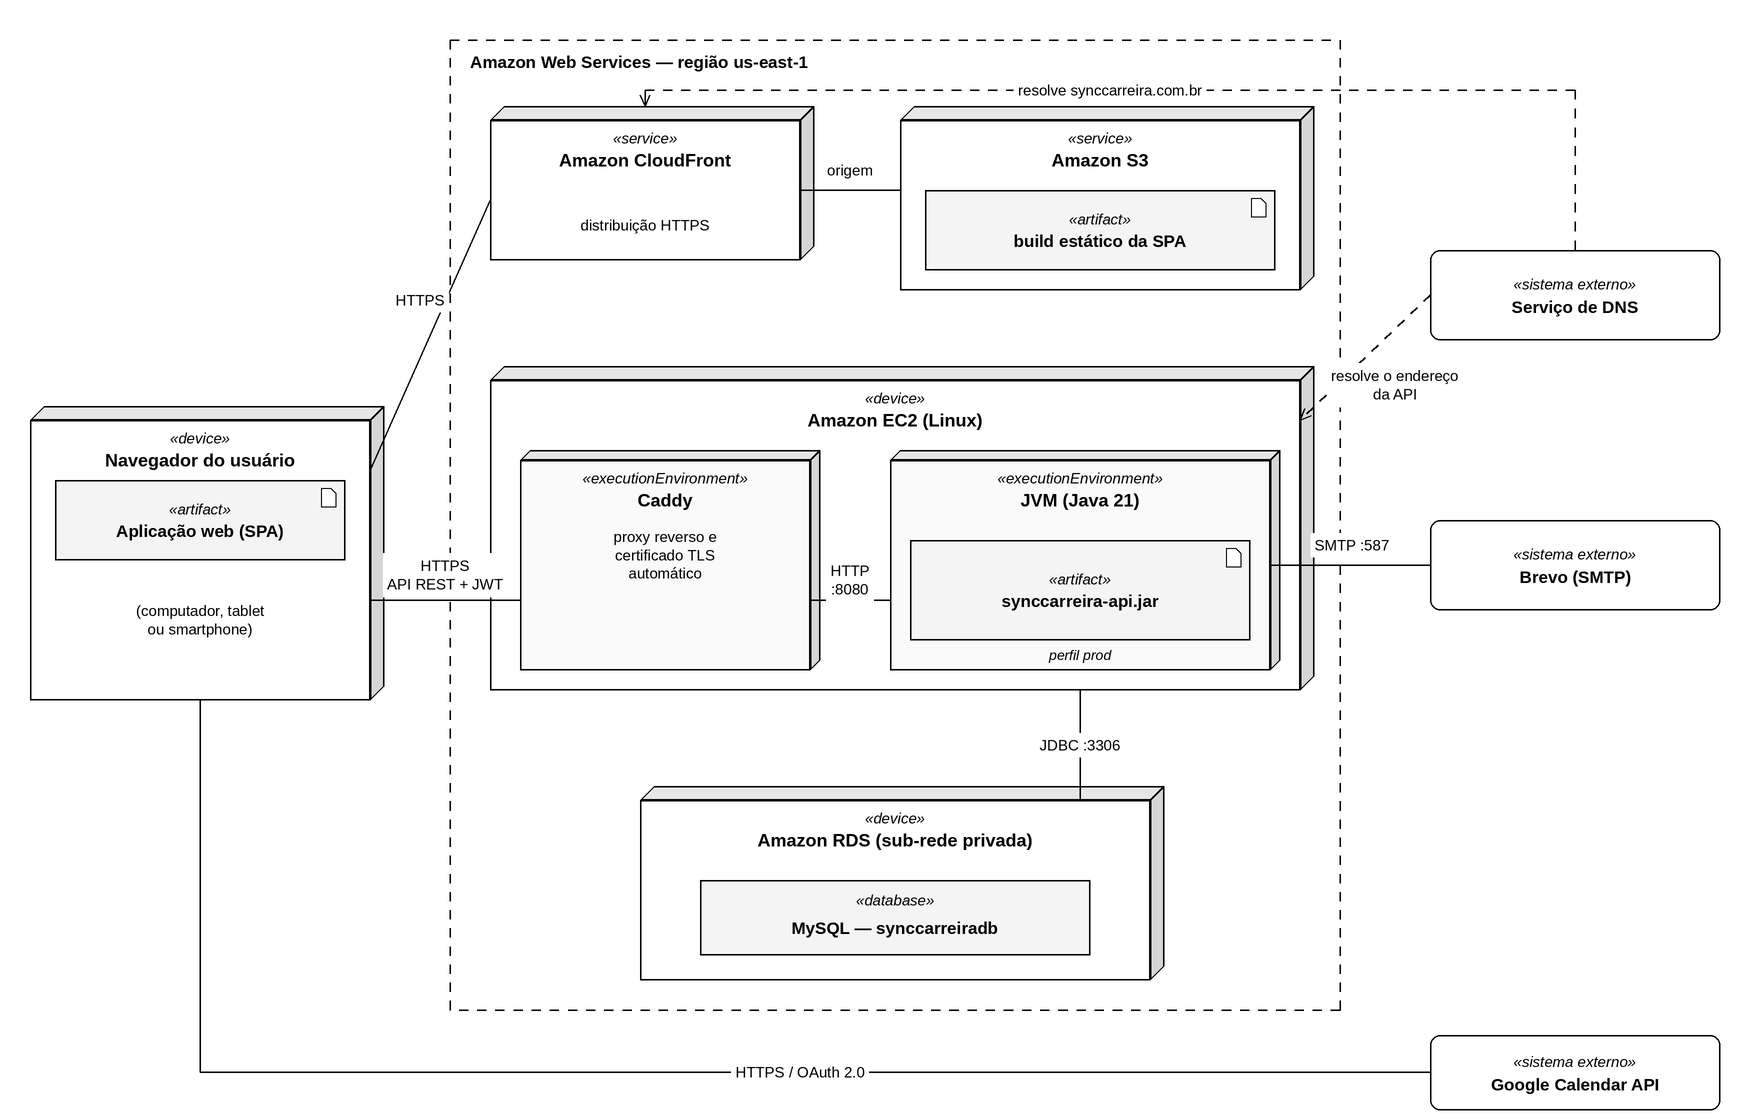
\includegraphics[width=\textwidth]{img/fig-cap5-implantacao.png}
    \legend{Fonte: Autoria própria (2026).}
\end{figure}

O ambiente de produção foi implantado na Amazon Web Services, na região us-east-1, e é acessado pelo domínio próprio do projeto, synccarreira.com.br, com a seguinte distribuição:

\begin{itemize}
  \item \textbf{aplicação \textit{web}}: os arquivos estáticos gerados no \textit{build} são armazenados em um \textit{bucket} do Amazon S3 e distribuídos pela rede de entrega de conteúdo Amazon CloudFront, que serve a aplicação por HTTPS no endereço synccarreira.com.br;
  \item \textbf{API}: executada em uma instância Amazon EC2 com sistema operacional Linux, na máquina virtual Java, com o perfil de produção; à frente da API, o servidor Caddy atua como \textit{proxy} reverso, recebendo as conexões HTTPS e encaminhando-as à aplicação, e obtém e renova automaticamente o certificado TLS;
  \item \textbf{banco de dados}: instância MySQL do Amazon RDS em sub-rede privada, acessível somente a partir da instância da API, carregada com o banco de questões, as subáreas do conhecimento e dados de teste;
  \item \textbf{nome de domínio}: os registros DNS do domínio synccarreira.com.br direcionam o endereço da aplicação \textit{web} para a distribuição do CloudFront e o endereço da API para o endereço público da instância EC2;
  \item \textbf{envio de e-mails}: realizado por meio do serviço de envio transacional Brevo, via SMTP, com remetente no domínio synccarreira.com.br.
\end{itemize}

As credenciais do servidor de e-mail e as demais configurações dependentes do ambiente são fornecidas por variáveis de ambiente da instância, e as alterações de esquema do banco são aplicadas pelos \textit{scripts} SQL versionados no repositório.

\section{Testes Realizados}

Os testes de \textit{software} têm como objetivo demonstrar que o programa faz o que se propõe a fazer e descobrir defeitos antes de seu uso, podendo ser conduzidos em diferentes níveis, desde componentes isolados até o sistema integrado \cite{sommerville2011}. No \textit{SyncCarreira}, os testes foram organizados em testes automatizados do servidor, análise estática contínua do código e testes manuais da API e da aplicação \textit{web}.

\subsection{Testes automatizados}

Os testes automatizados do servidor foram escritos com o JUnit 5 e somam 44 classes de teste, com 470 métodos de teste, organizadas nos mesmos pacotes do código de produção. O \autoref{quadro-testes} apresenta sua distribuição por tipo.

{\ABNTEXfontereduzida
\renewcommand{\arraystretch}{1.25}
\begin{xltabular}{\textwidth}{|>{\raggedright\arraybackslash}p{3.5cm}|>{\raggedright\arraybackslash}p{1.8cm}|>{\raggedright\arraybackslash}p{1.8cm}|>{\raggedright\arraybackslash}p{3.2cm}|>{\raggedright\arraybackslash}X|}
\multicolumn{5}{@{}c@{}}{\quadrolongocaption{Testes automatizados do servidor.}\label{quadro-testes}} \\[0.3em]
\hline
\textbf{Tipo} & \textbf{Classes} & \textbf{Métodos} & \textbf{Recursos} & \textbf{Objetivo} \\
\hline
\endfirsthead
\multicolumn{5}{@{}r@{}}{\textit{(continuação)}} \\
\hline
\textbf{Tipo} & \textbf{Classes} & \textbf{Métodos} & \textbf{Recursos} & \textbf{Objetivo} \\
\hline
\endhead
\multicolumn{5}{@{}r@{}}{\textit{(continua)}} \\
\endfoot
\endlastfoot
Unitários & 25 & 334 & JUnit 5 e Mockito & Verificar as regras de negócio dos serviços, o cálculo do leque, as entidades e os geradores de relatórios e documentos, com as dependências substituídas por objetos simulados. \\
\hline
De controlador & 14 & 119 & MockMvc & Verificar os recursos REST: códigos de situação, validação da entrada e formato das respostas e, em parte dos cenários, as restrições de acesso por perfil. \\
\hline
De repositório & 4 & 16 & H2 em memória & Verificar as consultas ao banco, em especial as consultas agregadas do painel. \\
\hline
De contexto & 1 & 1 & Spring Boot Test & Verificar a inicialização completa da aplicação. \\
\hline
\end{xltabular}
\legend{Fonte: Autoria própria (2026).}
}

Os testes são executados automaticamente no GitHub Actions a cada \textit{pull request} e a cada integração no ramo principal. O relatório de cobertura gerado pelo JaCoCo é enviado ao SonarCloud, que registrou cobertura de 89,3\% do código analisado, acima do mínimo de 80\% exigido para o código novo pelo critério de qualidade (\textit{quality gate}) padrão da ferramenta.

\subsection{Análise estática}

A cada integração, o SonarCloud realiza a análise estática do código e avalia o resultado em relação ao critério de qualidade. Na versão atual, o projeto encontra-se aprovado no \textit{quality gate}, com cobertura de 89,3\%, 0,4\% de código duplicado e nota A em segurança, em revisão de pontos sensíveis de segurança e em manutenibilidade. Em confiabilidade, a nota é C, com 47 apontamentos, predominantemente de severidade baixa. Os apontamentos da análise foram tratados como parte do fluxo de trabalho, a exemplo da substituição de injeção de dependência por atributo por injeção via construtor e da correção de uma possível referência nula no \textit{token} de autenticação. Os resultados completos da análise encontram-se no APÊNDICE B.

\subsection{Testes manuais}

Complementarmente, os fluxos de cada requisito foram exercitados manualmente no ambiente de desenvolvimento, com banco MySQL local, por meio de requisições à API. Esses testes revelaram problemas não cobertos pelos testes automatizados, apresentados no \autoref{quadro-testes-manuais} com as correções aplicadas.

{\ABNTEXfontereduzida
\renewcommand{\arraystretch}{1.25}
\begin{xltabular}{\textwidth}{|>{\raggedright\arraybackslash}p{5.9cm}|>{\raggedright\arraybackslash}X|}
\multicolumn{2}{@{}c@{}}{\quadrolongocaption{Problemas encontrados nos testes manuais e correções.}\label{quadro-testes-manuais}} \\[0.3em]
\hline
\textbf{Problema encontrado} & \textbf{Correção aplicada} \\
\hline
\endfirsthead
\multicolumn{2}{@{}r@{}}{\textit{(continuação)}} \\
\hline
\textbf{Problema encontrado} & \textbf{Correção aplicada} \\
\hline
\endhead
\multicolumn{2}{@{}r@{}}{\textit{(continua)}} \\
\endfoot
\endlastfoot
Requisições simultâneas de registro de respostas do mesmo aluno provocavam bloqueio mútuo no banco de dados e retornavam erro interno (500). & Repetição automática da operação em caso de bloqueio e conversão da falha persistente em resposta de conflito (409). \\
\hline
Corpo de requisição com JSON malformado retornava 422 com a mensagem técnica do interpretador de JSON. & Retorno de 400 com mensagem genérica; o código 422 permanece reservado para valores inválidos em JSON bem formado. \\
\hline
\end{xltabular}
\legend{Fonte: Autoria própria (2026).}
}

A aplicação \textit{web} foi verificada manualmente, com os três perfis de acesso, nos navegadores Google Chrome e Mozilla Firefox, abrangendo os fluxos de cada perfil e a adaptação da interface a diferentes larguras de tela.

\section{Resultados Obtidos}

A versão desenvolvida encontra-se em execução no ambiente de produção e contempla os três perfis de acesso previstos. O \autoref{quadro-situacao-rf} apresenta a situação de cada requisito funcional na versão atual.

{\ABNTEXfontereduzida
\renewcommand{\arraystretch}{1.25}
\begin{xltabular}{\textwidth}{|>{\raggedright\arraybackslash}p{1.8cm}|>{\raggedright\arraybackslash}p{4.7cm}|>{\raggedright\arraybackslash}p{2.5cm}|>{\raggedright\arraybackslash}X|}
\multicolumn{4}{@{}c@{}}{\quadrolongocaption{Situação dos requisitos funcionais.}\label{quadro-situacao-rf}} \\[0.3em]
\hline
\textbf{ID} & \textbf{Requisito} & \textbf{Situação} & \textbf{Observação} \\
\hline
\endfirsthead
\multicolumn{4}{@{}r@{}}{\textit{(continuação)}} \\
\hline
\textbf{ID} & \textbf{Requisito} & \textbf{Situação} & \textbf{Observação} \\
\hline
\endhead
\multicolumn{4}{@{}r@{}}{\textit{(continua)}} \\
\endfoot
\endlastfoot
RF-01 & Gestão de instituições & Atendido & Instituições e turmas. \\
\hline
RF-02 & Gestão de usuários e perfis & Atendido & Exclusão definitiva das contas; CRP ainda obrigatório no cadastro. \\
\hline
RF-03 & Painel de status por aluno & Atendido & Indicadores, progresso por trilha e filtros. \\
\hline
RF-04 & Alerta de necessidade de orientação & Atendido & Destaque no painel e mensagem eletrônica ao profissional. \\
\hline
RF-05 & Priorização de alunos em dúvida & Atendido & Filtro de alunos em dúvida no agendamento. \\
\hline
RF-06 & Curadoria de links externos & Atendido & Links gerais e por área do conhecimento. \\
\hline
RF-07 & Relatórios de turma e individuais & Atendido & Planilhas (.xlsx). \\
\hline
RF-08 & Agendamento de sessões & Atendido & Convite e videoconferência pelo Google Agenda. \\
\hline
RF-09 & Feedback personalizado & Atendido & Feedbacks de jornada e de sessão, com aviso por e-mail. \\
\hline
RF-10 & Jornada de 5 trilhas em ordem & Atendido & Quatro trilhas implementadas; a síntese final é registrada após a conclusão da última trilha. \\
\hline
RF-11 & Síntese ao final de cada trilha & Atendido & — \\
\hline
RF-12 & Leque de carreiras sugeridas & Atendido & Áreas em destaque, subáreas e carreiras. \\
\hline
RF-13 & Panorama da jornada & Atendido & — \\
\hline
RF-14 & Personalização de perfil & Atendido & Interesse por área do conhecimento. \\
\hline
RF-15 & Histórico de jornadas anteriores & Atendido & Consulta, exportação em PDF e nova jornada. \\
\hline
RF-16 & Agendamentos e feedbacks & Atendido & — \\
\hline
\end{xltabular}
\legend{Fonte: Autoria própria (2026).}
}

Quanto aos requisitos não funcionais, o \autoref{quadro-situacao-rnf} sintetiza a situação de cada um.

{\ABNTEXfontereduzida
\renewcommand{\arraystretch}{1.25}
\begin{xltabular}{\textwidth}{|>{\raggedright\arraybackslash}p{1.8cm}|>{\raggedright\arraybackslash}p{4.7cm}|>{\raggedright\arraybackslash}p{2.5cm}|>{\raggedright\arraybackslash}X|}
\multicolumn{4}{@{}c@{}}{\quadrolongocaption{Situação dos requisitos não funcionais.}\label{quadro-situacao-rnf}} \\[0.3em]
\hline
\textbf{ID} & \textbf{Requisito} & \textbf{Situação} & \textbf{Observação} \\
\hline
\endfirsthead
\multicolumn{4}{@{}r@{}}{\textit{(continuação)}} \\
\hline
\textbf{ID} & \textbf{Requisito} & \textbf{Situação} & \textbf{Observação} \\
\hline
\endhead
\multicolumn{4}{@{}r@{}}{\textit{(continua)}} \\
\endfoot
\endlastfoot
RNF-01 & Segurança (autenticação e autorização) & Atendido & Autorização por perfil e verificação de propriedade dos dados. \\
\hline
RNF-02 & Privacidade e proteção de dados & Parcial & Exclusão de dados implementada; dados sensíveis sem criptografia em repouso. \\
\hline
RNF-03 & Desempenho & Não medido & Sem medição formal do tempo de resposta. \\
\hline
RNF-04 & Usabilidade & Atendido & Interface responsiva, com atributos de acessibilidade. \\
\hline
RNF-05 & Disponibilidade & Não medido & Implantação em instância única, sem monitoramento de disponibilidade. \\
\hline
RNF-06 & Manutenibilidade & Atendido & Arquitetura em camadas, análise estática contínua e cobertura de testes de 89,3\%. \\
\hline
RNF-07 & Documentação de API & Atendido & Documentação gerada automaticamente (Swagger UI). \\
\hline
RNF-08 & Isolamento por instituição & Parcial & Isolamento de alunos, painel e sessões; links de informação compartilhados entre instituições. \\
\hline
\end{xltabular}
\legend{Fonte: Autoria própria (2026).}
}

Em relação aos objetivos do projeto, a solução estrutura a jornada do aluno em trilhas sequenciais com registro obrigatório de sínteses, fornece ao profissional de orientação o acompanhamento por turma sem exposição do conteúdo das respostas, sinaliza automaticamente os alunos que permanecem em dúvida, viabiliza o agendamento de sessões com convite automático, a curadoria de fontes externas, o envio de \textit{feedback} e a emissão de relatórios, e apresenta ao aluno um leque de possibilidades acompanhado de aviso explícito de que não se trata de diagnóstico. A gestão de múltiplas instituições com isolamento de dados e a exclusão definitiva de dados atendem às necessidades institucionais e às exigências da LGPD, com as ressalvas registradas na seção de limitações.

\section{Análise Financeira}

Como o desenvolvimento foi realizado pela equipe no âmbito do Projeto de Conclusão de Curso, sem remuneração, a análise financeira concentra-se no custo de operação da plataforma, isto é, no valor que a instituição parceira deverá custear mensalmente para mantê-la em funcionamento na configuração atual.

A estimativa considera os preços sob demanda da região us-east-1 da Amazon Web Services \cite{aws2026ec2preco, aws2026ebspreco, aws2026rdspreco, aws2026cloudfrontpreco, barr2023ipv4}, um mês de 730 horas de funcionamento contínuo e a cotação de referência de R\$ 5,20 por dólar \cite{mercadohoje2026dolar}. Não foram considerados os créditos e cotas do nível gratuito da AWS, que dependem da data de criação da conta e reduzem o custo apenas nos primeiros meses, nem os tributos incidentes sobre pagamentos internacionais. O \autoref{quadro-custos} apresenta a memória de cálculo.

{\ABNTEXfontereduzida
\renewcommand{\arraystretch}{1.25}
\begin{xltabular}{\textwidth}{|>{\raggedright\arraybackslash}p{3.7cm}|>{\raggedright\arraybackslash}p{4.2cm}|>{\raggedright\arraybackslash}X|>{\raggedright\arraybackslash}p{2.8cm}|}
\multicolumn{4}{@{}c@{}}{\quadrolongocaption{Estimativa do custo mensal de operação.}\label{quadro-custos}} \\[0.3em]
\hline
\textbf{Item} & \textbf{Configuração considerada} & \textbf{Base de cálculo} & \textbf{Custo mensal (R\$)} \\
\hline
\endfirsthead
\multicolumn{4}{@{}r@{}}{\textit{(continuação)}} \\
\hline
\textbf{Item} & \textbf{Configuração considerada} & \textbf{Base de cálculo} & \textbf{Custo mensal (R\$)} \\
\hline
\endhead
\multicolumn{4}{@{}r@{}}{\textit{(continua)}} \\
\endfoot
\endlastfoot
Amazon EC2 & Instância t3.micro (2 vCPU, 1 GiB de memória) & 730 h $\times$ US\$ 0,0104/h = US\$ 7,59 & 39,47 \\
\hline
Amazon EBS & Volume gp3 de 8 GB da instância & 8 GB $\times$ US\$ 0,08/GB = US\$ 0,64 & 3,33 \\
\hline
Endereço IPv4 público & Um endereço associado à instância & 730 h $\times$ US\$ 0,005/h = US\$ 3,65 & 18,98 \\
\hline
Amazon RDS for MySQL & Instância db.t3.micro, Single-AZ & 730 h $\times$ US\$ 0,017/h = US\$ 12,41 & 64,53 \\
\hline
Armazenamento do RDS & 20 GB em SSD de uso geral (gp2) & 20 GB $\times$ US\$ 0,115/GB = US\$ 2,30 & 11,96 \\
\hline
Amazon S3 e CloudFront & Arquivos estáticos da aplicação \textit{web} & Volume dentro das cotas gratuitas permanentes do CloudFront; armazenamento inferior a US\$ 0,01 & 0,00 \\
\hline
Domínio synccarreira.com.br & Registro anual no Registro.br & R\$ 40,00 por ano $\div$ 12 \cite{homehost2026dominio} & 3,33 \\
\hline
Brevo & Plano pago de envio de e-mails transacionais & Valor mensal contratado: R\$ 40,00 & 40,00 \\
\hline
\textbf{Total} &  &  & \textbf{181,60} \\
\hline
\end{xltabular}
\legend{Fonte: Autoria própria (2026).}
}

O custo estimado de operação é, portanto, de aproximadamente R\$ 181,60 por mês, ou R\$ 2.179,20 por ano. O banco de dados gerenciado responde por cerca de 42\% desse valor; a instância da API, somada ao seu armazenamento e ao endereço público, por cerca de 34\%; e o serviço de envio de e-mails, por cerca de 22\%. Como a plataforma é dimensionada para o volume de uso de uma instituição parceira, o crescimento do número de instituições e de alunos tende a exigir instâncias de maior capacidade, com aumento proporcional dos custos de computação e de banco de dados. Em contrapartida, a contratação de instâncias reservadas ou de planos de economia da AWS, com compromisso de um ou três anos, permite reduzir o custo da capacidade computacional em relação aos preços sob demanda.

\section{Limitações da Implementação}

A versão atual apresenta as seguintes limitações conhecidas:

\begin{itemize}
  \item \textbf{registro profissional}: o número de registro no Conselho Regional de Psicologia permanece obrigatório no cadastro, o que impede o cadastro de mentores sem registro;
  \item \textbf{criptografia de dados sensíveis}: respostas, sínteses e perfis são armazenados sem criptografia em repouso; apenas as senhas são protegidas por função de \textit{hash};
  \item \textbf{chave de assinatura dos \textit{tokens}}: o par de chaves é gerado em memória a cada inicialização da API, o que invalida as sessões abertas a cada reinício e impede a execução de múltiplas instâncias com \textit{tokens} compartilhados;
  \item \textbf{armazenamento do \textit{token}}: o \textit{token} de acesso é mantido no armazenamento local do navegador, acessível a \textit{scripts} em caso de vulnerabilidade de injeção de código;
  \item \textbf{validade do contrato}: o contrato vencido do profissional de orientação não impede seu acesso ao sistema;
  \item \textbf{links de informação}: não são vinculados a uma instituição e, por isso, são exibidos a alunos de todas as instituições;
  \item \textbf{gestão de senhas}: não há recuperação de senha pelo próprio usuário nem reenvio do \textit{link} de primeiro acesso; o usuário é orientado a procurar o Administrador;
  \item \textbf{consulta ao banco de questões}: a consulta pelo profissional de orientação está disponível na API, mas não possui tela na aplicação \textit{web};
  \item \textbf{consentimento}: o fluxo de aceite do termo de consentimento previsto no Documento de Requisitos não foi implementado;
  \item \textbf{apontamentos da análise estática}: permanecem em aberto dois apontamentos de segurança de severidade alta e os apontamentos de confiabilidade que resultam na nota C nesse critério;
  \item \textbf{infraestrutura}: a API é executada em instância única, sem redundância, balanceamento de carga ou monitoramento, e a implantação é realizada manualmente, sem fluxo de entrega contínua; o desempenho e a disponibilidade não foram medidos;
  \item \textbf{testes da aplicação \textit{web}}: a aplicação \textit{web} não possui testes automatizados, e sua verificação depende de testes manuais.
\end{itemize}
